\chapter{Numerical Method}
\label{chapter2}

%--------------------------------------
\section{Mathematical Models and Numerical Method}
\label{sec:equations}

\subsection{Linear Elastic Equation and Weak Galerkin Method}
Consider an elastic body subject to an exterior force $ \mathbf{f} $, and denote the computational domain as $ \Omega $ and its continuous boundary as $ \Gamma = \partial \Omega $. The governing elasticity equation can be written as

\begin{equation}
\nabla \cdot \sigma(\mathbf{u}) = \mathbf{f}, \qquad in \quad \Omega 
\end{equation}
\begin{equation}
\mathbf{f} = \hat{\mathbf{f}}, \qquad in \quad \Omega
\end{equation}
\begin{equation}
\mathbf{u} = \hat{\mathbf{u}}, \qquad on \quad \Gamma
\end{equation}
where $ \sigma(\mathbf{u}) $ is the symmetric Cauchy stress tensor. For linear, isotropic and homogeneous materials, the stress-strain relation is
\begin{equation}
\sigma(\mathbf{u}) = 2 \mu \varepsilon(\mathbf{u}) + \lambda (\nabla \cdot \mathbf{u}) \mathbf{I}
\end{equation}
where $ \varepsilon(\mathbf{u}) = \frac{1}{2} (\nabla \mathbf{u} + \nabla \mathbf{u}^{T}) $, $ \mu $ and $ \lambda  $ are Lame indices which can be written as 
\begin{equation}
\lambda = \frac{E\mu }{(1 + \mu) (1 - 2\mu)}
\end{equation}
\begin{equation}
\mu = \frac{E}{2(1+\mu)}
\end{equation}
where $ E $ is the elasticity modulus and $ \mu $ is the Poisson's ratio.



The weak function on the domain is $ \mathbf{u} = \{\mathbf{u}_0, \mathbf{u}_b \}, \quad \mathbf{u}_0 \in L^{2} (T) $. The first function $ \mathbf{u}_0 $  represents the interior domain of the function $ \mathbf{u} $ . The second function $ \mathbf{u}_b $ represents the value of function $ \mathbf{u} $ on the boundary of domain $ T $ . The key notion is that the basis functions of $ \mathbf{u}_0 $  and $ \mathbf{u}_b $  are independent with each other . The weak function is defined as
\begin{equation}
V_{h} = \{ \mathbf{v} = \{ \mathbf{v}_0, \mathbf{v}_b \} : \mathbf{v}_0 \in P_{j} (T^0), \mathbf{v}_b \in P_{l}(e), e \subset \partial T\}
\end{equation}

The key of the weak Galerkin method is to approximate the solution in the weak discrete space $ S(T) $. The discrete weak gradient $ \nabla_{w} \mathbf{u} \in [P_{r} (T)]^{d} $ for $ \mathbf{u} \in V_{h} $ on each element $ T $:
\begin{equation}
(\nabla_w \mathbf{u}, \mathbf{q})_{T} = - (\mathbf{u}_0, \nabla \cdot \mathbf{q})_{T} + \langle \mathbf{u}_b, q \cdot \mathbf{n} \rangle_{\partial T}
\end{equation}

For the discrete weak divergence, $ \nabla_{w} \cdot \mathbf{u} \in [P_{r} (T)]^{d} $ is defined
\begin{equation}
(\nabla_w \cdot \mathbf{u}, \mathbf{q})_{T} = - (\mathbf{u}_0, \nabla  \mathbf{q})_{T} + \langle \mathbf{u}_b \cdot \mathbf{n}, q  \rangle_{\partial T}
\end{equation}

Then we can define the weak strain tensor by using the weak gradient
\begin{equation}
\varepsilon_{w} (\mathbf{u})  = \frac{1}{2} (\nabla_w  \mathbf{u} + \nabla_w  \mathbf{u}^T)
\end{equation}

Analogously, we can define the weak stress tensor as
\begin{equation}
\sigma_{w} ( \mathbf{u}) = 2 \mu \varepsilon_{w} ( \mathbf{u}) + \lambda (\nabla_w \cdot  \mathbf{u}) \mathbf{I}
\end{equation}

The bilinear form of governing equation of continuous Galerkin method is following
\begin{equation}
a( \mathbf{u},  \mathbf{v}) = ( \mathbf{f},  \mathbf{v})
\end{equation}

In WG method, to complete the elemental stiffness matrix, we need the stabilizer to connect the interior and boundary unknown variables. The matrix form of governing equation is
\begin{equation}
a( \mathbf{u}_w,  \mathbf{v}_w) + s( \mathbf{u},  \mathbf{v}) = ( \mathbf{f},  \mathbf{u})
\end{equation}
the term $ s( \mathbf{u},  \mathbf{v}) $ is a stabilizer enforcing a weak continuity which measures the discontinuity of the finite element solution. The governing equation in weak form can be introduced by two bilinear equations
\begin{equation}
s( \mathbf{u},  \mathbf{u}) = \sum_{T\in \Omega}^{N} h_{T}^{-1} \langle Q_{b}  \mathbf{u}_0 -  \mathbf{u}_b, Q_b  \mathbf{v}_0 -  \mathbf{v}_b \rangle_{\partial T}
\end{equation}
where $ Q_b $ is the projection from the interior unknown variables to boundary unknown variables. Commonly it is taken as $ 1 $. The matrix form of governing equation is assembled as
\begin{equation}
a( \mathbf{u}_w,  \mathbf{u}_w) = \sum_{T \in \Omega}^{N} 2(\mu \varepsilon_w ( \mathbf{u}), \varepsilon_w ( \mathbf{v}))_T + \sum_{T \in \Omega}^{N}(\lambda \nabla \cdot \mathbf{u}, \nabla_w \cdot \mathbf{v})_T
\end{equation}


%--------------------------------------
\section{Existing Numerical Methods Review}
In this section, we present and analyze several most widely used numerical method for solving finite element problems. The details of each method are presented in the following subsections.
 
\subsection{Classic Continuous Galerkin Finite Element Method}
Back to 1950s and 1960s, finite element method is invented to solve complex elasticity and structural analysis engineering problems in mechanical and aeronautical field. A. Hrennikoff \cite{hrennikoff1941solution}, R. Courant \cite{courant1994variational} and K.Feng \cite{babuvska2001finite} are the earliest pioneers who established this subject. FEM is then proposed as a systematic numerical method to solve variety of partial differential equations. The core characteristic of FEM is that it employs mesh discretization to divide a continuous computational domain. Therefore, a big problem is then converted to a set of discrete small problems. That is the source of finite element. Each element represents a small piece of computational sub-domain.

FEM is an efficient solution to solve partial differential equations. It converts the original partial differential equation to an equivalent bilinear form as the weak function. Then we partition the computational domain into polygon meshes. In each mesh element, we construct the finite element space. The bilinear form is discretized into a summation of finite elemental matrices. The solution is approximated based on the calculation of assembled matrix. More details can be found in \cite{zienkiewicz1977finite, ciarlet2002finite, hughes2012finite, reddy1993introduction}.

The variational formulation is derived from the governing equation. It determines the characteristic of the finite element method. To obtain the variational form, mathematicians derived several different paths such as Galerkin method, the discontinuous Galerkin method, mixed method, etc. In this chapter, we introduce two most popular method, DG and MFEM. The WG methods is inspired from these two method and shares many similarities with them. 

\subsection{Discontinuous Galerkin Finite Element Method}

We shall go through a simple example to review the common features of FEM and the new feature of DG-FEM.

We have a 1-dimensional convection equation with domain $ [0, \pi] $

\begin{equation}
a \frac{du}{dx} = cos(x)
\end{equation}

the exact solution is
\begin{equation}
u = \frac{sin(x)}{a}
\end{equation}
where the Dirichlet boundary condition is applied on both end.

For the classic CG FEM, we shall first apply the basis function $ \phi_{i} $ on each element. The solution becomes as
\begin{equation}
u(x) = \sum_{i = 1}^{N} \phi_{i} (x) U_{i}
\end{equation}

We integrate the governing equation and obtain the weak form
\begin{equation}
\int_{\Omega} a \frac{du}{dx} \phi_{i} dx = \int_{\Omega} cos(x) \phi_i dx
\end{equation}

Then we apply integration by parts
\begin{equation}
-\int_{\Omega} a u \phi_{i, x} dx + [a u \phi_{i}]^{right}_{left} = \int_{\Omega} cos(x) \phi_{i} dx
\end{equation}

Discrete form of the continuous unknown function is
\begin{equation}
u(x) = \sum_{i = 1}^{N} \phi_{i}(x) U_{i}
\end{equation}

So we obtain the new governing equation in matrix form
\begin{equation}
-\sum_{i = 1}^{N} U_{i} a \int_{\Omega} \phi_{i}\phi_{j,x} dx + BC = \int_{\Omega} cos(x) \phi_{j} dx
\end{equation}

The linear system is simplified as
\begin{equation}
\mathbf{A} \mathbf{x} = \mathbf{b}
\end{equation}

In DG-FEM, there is no continuity constraint between element. In another word, the basis functions in the computational domain is discontinuous.

The discretized governing equation in matrix form is
\begin{equation}
a \int_{\Omega} \frac{du}{dx} \phi_{i}  dx = \int_{\Omega} cos(x) \phi_{i} dx
\end{equation}

For the integration by parts, the equation is written in
\begin{equation}
\sum_{j} \int_{j} a \frac{du}{dx} \phi_{i} dx = \sum_{j} \int_{j} cos(x) \phi_{i} dx
\end{equation}

Then we apply the integration by parts
\begin{equation}
\sum_{j} \{ -\int_{j} a u \phi_{i, x} dx + [(a u)\phi_{i}]^{j + \frac{1}{2}}_{j - \frac{1}{2}} \} = \sum_{j} \int_{j} cos(x) \phi_{i} dx
\end{equation}

For every element, we have the elemental matrix form 
\begin{equation}
-\int_{j} au\phi_{j,x} dx + [(au)\phi_{i}]^{j + \frac{1}{2}}_{j - \frac{1}{2}} = \int_{j} cos(x) \phi_{j} dx
\end{equation}

A penalty term is required in the above equation representing a jump of the interface value. There are several methods to calculate it. Upwinding method is a common useful tool to calculate the $ u $ value on the interface. Comparing to the CG method, the DG method introduces additional DOFs to maintain the continuity as jump penalty term. 

There are several widely applied iterative schemes such as block Jacobi, Conjugate Gradient method are stable for elements with high order polynomials. Domain decomposition is compatible with the DG method as parallel computing scheme.


\subsection{Mixed Finite Element Method}

The mixed finite element method is a new type of the FEM in which an extra independent variable is introduced which discretization of a partial differential equation. It is characterized by a variational equation. Usually, the extra variables are constrained by an external vector, Lagrange multiplier. The main difference between FEM and mixed FEM is that the changing of bilinear form of governing equation. The mixed FEM has an advantage on computing the elasticity equation and the stress and strain field. 

To illustrate the mixed FEM, a simple elliptic equation is
\begin{equation}
- \nabla \cdot (a \nabla u) = f \quad in \quad \Omega
\end{equation}

\begin{equation}
u = 0 \quad on \quad \partial \Omega
\end{equation}

we shall introduce an vector $ \mathbf{G} $ that

\begin{equation}
\mathbf{G} = -a \nabla u
\end{equation}

the elliptic problem then can be decomposed into a first order linear system that
\begin{equation}
\mathbf{G} + a \nabla u = 0 \quad in \quad \Omega
\end{equation}

\begin{equation}
\nabla \cdot \mathbf{G} = f \quad in  \quad \Omega 
\end{equation}

\begin{equation}
u = 0 \quad  on  \quad \partial \Omega 
\end{equation}

we can rewrite the first equation as
\begin{equation}
a^{-1} \mathbf{G} + \nabla u = 0 \quad in \quad \Omega 
\end{equation}

then we apply the integration by parts
\begin{equation}
\int_{\Omega} a^{-1} \mathbf{G} \cdot \mathbf{v} d\Omega - \int_{\Omega} c \nabla \cdot \mathbf{v} d\Omega = 0 \quad \mathbf{v} \in H(div, \Omega)
\end{equation}
$ H(div, \Omega) $ represents the integral function is defined in Hilbert space as $ \Omega $.

\begin{equation}
\int_{\Omega} \psi \nabla \cdot \mathbf{G} d\Omega = \int_{\Omega} f \psi d\Omega 
\end{equation}

where 
\begin{equation}
H(div, \Omega) = \{\mathbf{v} \in L^{2}(\Omega)^{d} : \nabla \cdot \mathbf{v} \in L^{2}(\Omega) \}
\end{equation}

We use the Raviart-Thomas spaces to define a generic element $ T \in \Omega $
\begin{equation}
RT_{k} = (P_{k})^{d} + xP_{k}
\end{equation}
where $ k  $ is the order of polynomials degrees.

the variational function $ \tilde{G} $ and $ \mathbf{u} $ can be approximated by 
\begin{equation}
\tilde{G} = \sum_{i = 1}^{N}g_{i} \mathbf{v}_{i}
\end{equation}

\begin{equation}
\mathbf{u} = \sum_{i = 1}^{N} u_{i} \psi_{i}
\end{equation}
both $ \mathbf{v} $ and $ \phi_{i} $ are vector basis functions. If we consider the $ RT_0 $ space, 
\begin{equation}
\mathbf{v} = \begin{pmatrix}
ax + b \\ ay + c\\
\end{pmatrix}
\end{equation}

for each element $ T_{i} , (i = 1, 2, 3)$
\begin{equation}
v_{i} = \begin{pmatrix}
a_{i} x + b_{i} \\ a_{i} y + c_{i}\\
\end{pmatrix}
\end{equation}

the above equation follows the Kronecker property \cite{davio1981kronecker}

\begin{eqnarray}
&&\int_{T} v_{i} \cdot \mathbf{n} dS = \int_{T} (ax + b)n_{x} + (ay + c)n_{y} dS\\
&=& a\int_{x_1}^{x_2} (x_1 n_x + y_1 n_y) \frac{1}{n_y} dx + \int_{x_1}^{x_2}(bn_x + cn_y) \frac{1}{n_y} dx  \\
&=& a(x_1 n_x + y_1 n_y) \frac{x_1 - x_2}{n_y} + (bn_x + cn_y) \frac{x_1 - x_2}{n_y} \\
&=& \delta_{ij}
\end{eqnarray}

Then we apply the divergence theorem, we have
\begin{eqnarray}
\int_{T} \nabla \cdot \mathbf{v} dx dy & = & \int_{T} (\frac{\partial \mathbf{v}}{\partial x} + \frac{\partial \mathbf{v}}{\partial y}) dS\\
&=& \int_{T} 2a dS \\
&=& 2a |T_{i}|
\end{eqnarray}


%---------------------------
\section{Weak Galerkin Finite Element Methods}

\subsection{Preliminary}
In this section, all computation is in Sobolev space\cite{brenner2007mathematical, ciarlet2002finite}. The Lipschitz boundary is in open area $ D \subset R^{d} $, $ d = 2, 3 $. The inner product is defined as
\begin{equation}
|v|_{s, D} = \begin{pmatrix}
\sum_{|\alpha| = s} \int_{D} |\partial^{2} v|^{2} dD
\end{pmatrix}^{1/2}
\end{equation}

where
\begin{equation}
\alpha = (\alpha_{1}, \dots, \alpha_{d})
\end{equation}
\begin{equation}
|\alpha| = \alpha_{1} + \cdots + \alpha_d
\end{equation}

The definition of divergence is defined by
\begin{equation}
H(div; D) = \{ \mathbf{v} : \mathbf{v} \in [L^{2}(D)]^{d}, \nabla \cdot \mathbf{v} \in L^{2}(D) \}
\end{equation}
the norm is defined as
\begin{equation}
||\mathbf{v}||_{H(div, D)} = (||\mathbf{v}||^{2}_{D} + ||\nabla \cdot \mathbf{v}||^{2}_{D})^{1/2}
\end{equation}

the curl of $ H(curl; D) $ in $ L^{2}(D) $ is defined as
\begin{equation}
H(curl; D) = \{\mathbf{v} : \mathbf{v} \in [L^{2}(D)]^{d}, \nabla \times \mathbf{v} \in L^{2}(D)\}
\end{equation}
the norm of it is defined as
\begin{equation}
||\mathbf{v}||_{H(curl; D)} = (||\mathbf{v}||^{2}_{D} + ||\nabla \times \mathbf{v}||^{2}_{D})^{1/2}
\end{equation}

\subsection{Weak operators}

Let's assume that $ T \subset R^{d} $ is an arbitrary polygon domain, the boundary is $ \partial T $. The weak function in the domain is $ v = \{v_{0}, v_{b}\} $, so that $ v_{0} \in L^{2}(T) $ and $ v_{b} \in L^{2} (\partial T) $. The $ v_{0} $ represents the unknown variable vector belongs to the interior domain, and $ v_{b} $ represents the unknown variable vector along the boundary of $ T $. The keynote is that the $ v_{0}  $ is independent with $ v_{b} $ on $ \partial T $. The weak space for all $ T $ is $ S(T) $

\begin{equation}
S(T) = \{ v = \{v_{0}, v_{b}\} : v_{0} \in L^{2}(T), v_{b} \in L^{2} (\partial T) \}
\end{equation}

Now we define some commonly used weak operators

The weak gradient operator, for any $ v \in S(T) $, the weak gradient of $ v $ is $ \nabla_{w} v $
\begin{equation}
( \nabla_{w} v, \mathbf{q} )_{T} = -(v_{0}, \nabla \cdot \mathbf{q})_{T} + \langle v_{b}, \mathbf{q} \cdot \mathbf{n} \rangle_{\partial T}
\end{equation}

the discrete weak gradient operator is $ \nabla_{w, r} v $
\begin{equation}
(\nabla_{w,r} v, \mathbf{q})_{T} = -(v_{0}, \nabla \cdot \mathbf{q})_{T} + \langle v_{b}, \mathbf{q} \cdot \mathbf{n} \rangle_{\partial T}
\end{equation}
where
\begin{equation}
V(T) = \{ \mathbf{v} = \{  \mathbf{v}_{0}, \mathbf{v}_{b} \} : \mathbf{v}_{0} \in [L^{2} (T)]^{d}, \mathbf{v}_{b} \in [L^{2} (\partial T)]^{d} \}
\end{equation}

The weak divergence operator, for any $ v \in S(T) $, is $ \nabla \cdot \mathbf{v} $
\begin{equation}
\langle \nabla_{w} \cdot \mathbf{v}, \varphi \rangle_{T} = -(\mathbf{v}_{0}, \nabla \varphi)_{K} + \langle \mathbf{v}_{b} \cdot \mathbf{n}, \varphi \rangle_{\partial T}
\end{equation}

the discrete weak divergence operator is 
\begin{equation}
(\nabla_{w, r, T} \cdot \mathbf{v}, \varphi)_{T} = -(\mathbf{v}_{0}, \nabla \varphi)_{T} + \langle \mathbf{v}_{b} \cdot \mathbf{n}, \varphi \rangle_{\partial T}
\end{equation}

the curl operator , for any $ v \in S(T) $, is $ \nabla_{w} \times \mathbf{v}$ which is defined as 
\begin{equation}
\langle \nabla_{w} \times \mathbf{v}, \varphi \rangle_{T} = (\mathbf{v}_{0}, \nabla \times \varphi)_{T} - \langle \mathbf{v}_{b} \times \mathbf{n}, \varphi \rangle_{\partial T}
\end{equation}

the discrete weak divergence operator is 
\begin{equation}
(\nabla_{w, r, T} \times \mathbf{v}, \varphi)_{T} = (\mathbf{v}_{0}, \nabla \times \varphi)_{T} - \langle \mathbf{v}_{b} \times \mathbf{n}, \varphi \rangle_{\partial K}
\end{equation}

\subsection{Weak Galerkin method for second order elliptic equation}
In this section, we use the weak operators to solve second order elliptic equation. In domain $ \Omega $, we have the equation in form
\begin{equation}
- \nabla \cdot (a \nabla u) = f
\end{equation}

Considering the Dirichlet boundary condition, we have
\begin{equation}
u = -g, \quad on \quad \partial \Omega
\end{equation}

For Neumann boundary condition, we have
\begin{equation}
(a \nabla u) \cdot \mathbf{n} = -g, \quad on \quad \partial \Omega
\end{equation}

The primal formulation for Dirichlet boundary condition is 
\begin{equation}
(a \nabla u, \nabla v) = (f, v)
\end{equation}

For Neumann boundary condition
\begin{equation}
(a \nabla u, \nabla v) = (f, v) - \langle g, v \rangle_{\partial \Omega}
\end{equation}

The Primal-Mixed formulation is to make $ \mathbf{q} = -a \nabla u $, the elliptic equation is 
\begin{equation}
a^{-1}\mathbf{q} + \nabla u = 0,
\end{equation}

\begin{equation}
\nabla \cdot \mathbf{q} = f.
\end{equation}

we choose assistant function $ \mathbf{p} \in [L^{2}(\Omega)]^{d} $, the bilinear form is
\begin{equation}
(a^{-1} \mathbf{q}, \mathbf{p}) + (\nabla u, \mathbf{p}) = 0;
\end{equation}

for any $ v \in H_{0}^{1} (\Omega) $
\begin{equation}
(\mathbf{q}, \nabla v) = -(f, v)
\end{equation}

For Dirichlet boundary condition, $ u \in H^{1}(\Omega) $, $ \mathbf{q} \in [L^{2} (\Omega)]^{d} $, so that we enforce the boundary condition $ u = -g  $ on $ \partial \Omega $
\begin{equation}
(a^{-1}, \mathbf{q}, \mathbf{p}) + (\nabla u, \mathbf{p})
\end{equation}

\begin{equation}
(\mathbf{q}, \nabla v) = -(f, v),
\end{equation}

for Neumann boundary condition
\begin{equation}
(a^{-1} \mathbf{q}, \mathbf{p}) + (\nabla u, \mathbf{p}) = 0,
\end{equation}

\begin{equation}
(\mathbf{q}, \nabla v) = \langle g, v \rangle_{\partial \Omega} - (f, v),
\end{equation}

Let's define the weak function on each element space
\begin{equation}
S(k, T) = \{ v = \{ v_{0}, v_{b} \} : v_{0} \in P_{k} (T), v_{b}|_{e} \in P_{k} \}
\end{equation}
where $ k $ is the order of polynomial for each function, and $ e $ is the boundary edge of each element.

The weak space $ S_{h} $ is defined as
\begin{equation}
S_{h} = \{ v = \{ v_{0}, v_{b} \} : v |_{T} \in S(k, T), v_{b} |_{\partial T} \}
\end{equation}

for each element $ T $, we use $ Q_{0} $ to represent the $ L^{2} $ projection from $ L^{T} $ to $ P_{k}(T) $ and $ Q_{b} $ is the $ L^{2} $ projection from $ L^{2}(T) $ to $ P_{k}(\partial T) $. The local weak discrete space $ Q_{h} $ is
\begin{equation}
Q_{h} v = \{ Q_{0} v_{0}, Q_{b}, v_{b} \}
\end{equation}

in space $ S_{h} $ we have the bilinear form
\begin{equation}
a(u, v) = \sum (a \nabla_{w} u, \nabla_{w} v)_{T}
\end{equation}

To connect the two independent spaces, interior and boundary, a stabilizer is introduced. The stabilizer describes the difference of boundary values and the projected interior value to the boundary. Since the interior space and boundary space is independent, two sets of basis functions are applied independently. When we project the value from interior basis function to boundary basis function, the two values are different even though they share the same location. The stabilizer is a boundary integral which measure the difference and connect the spaces.

\begin{figure}[h]
	\centering
	\begin{tabular}{c}
		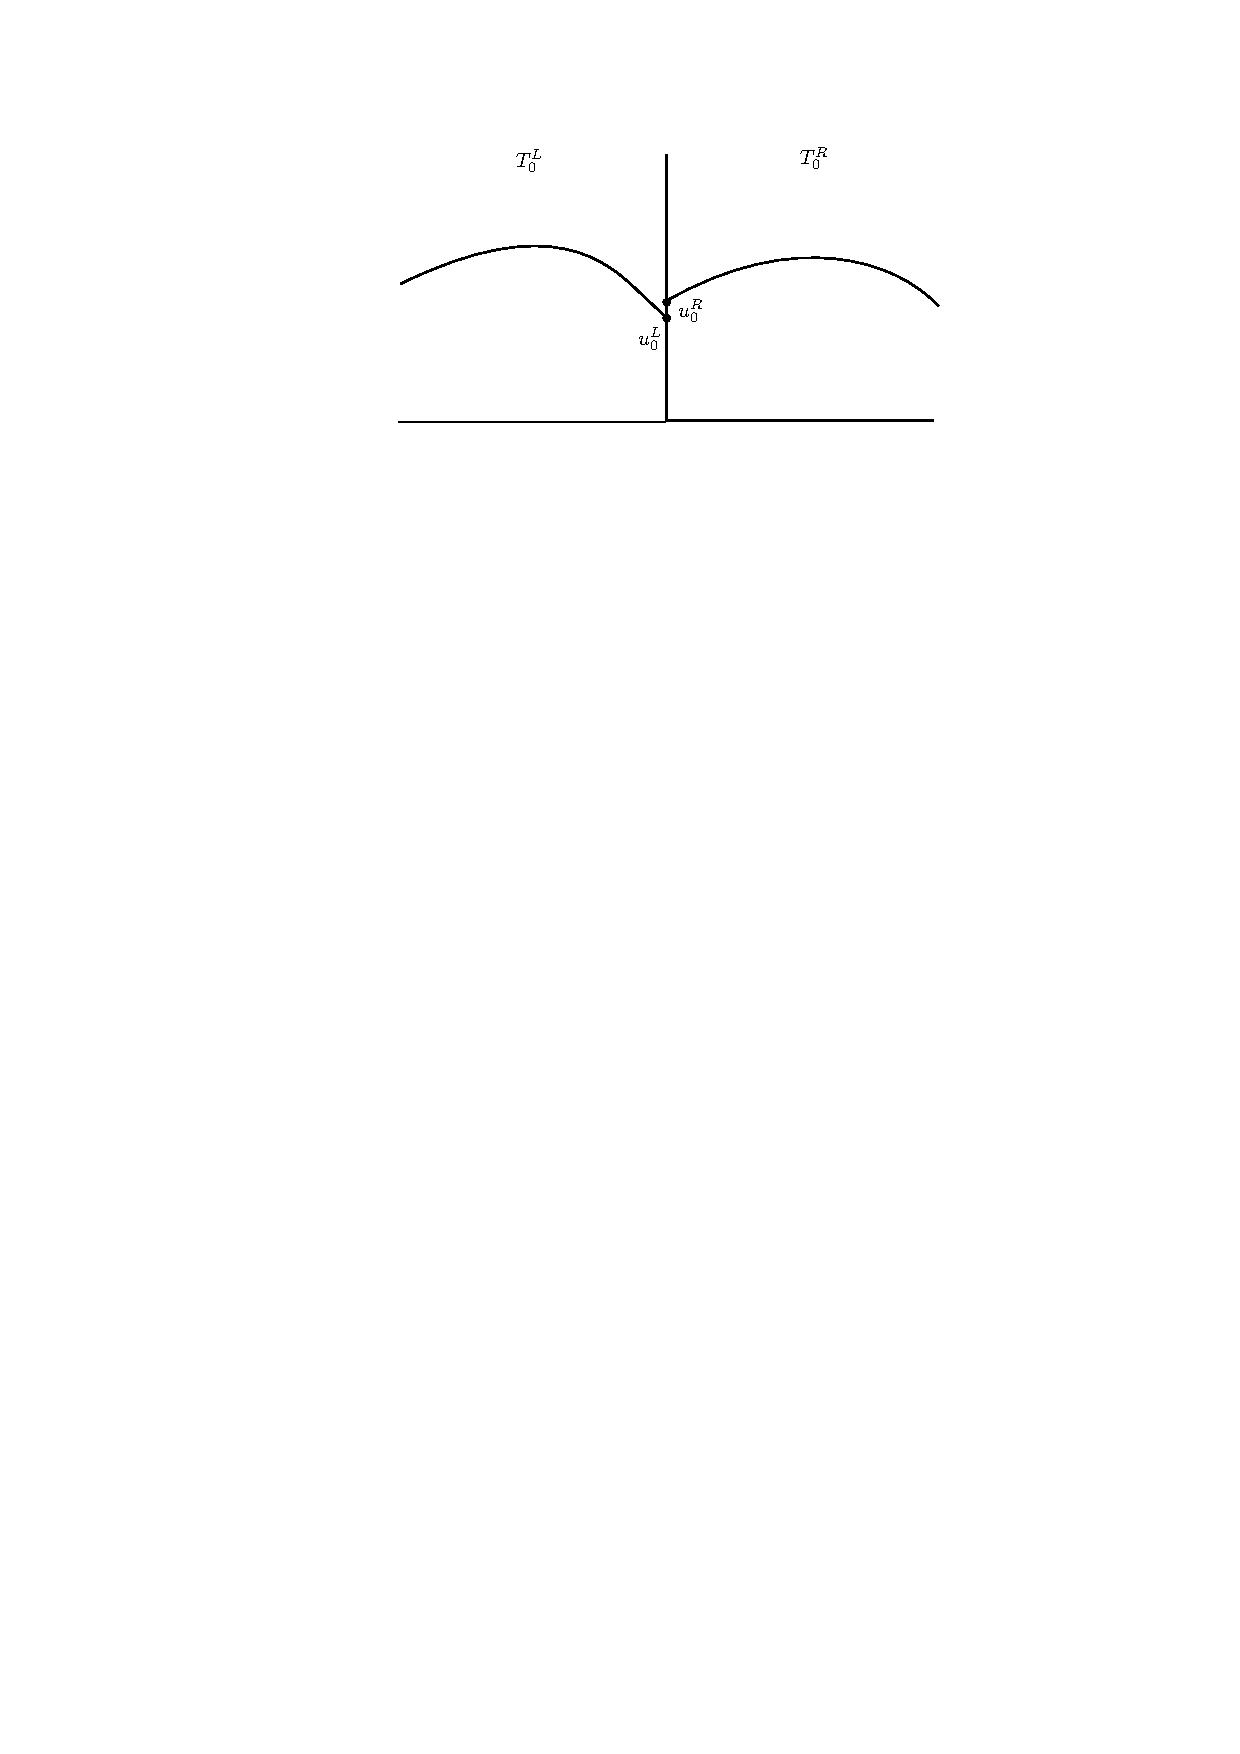
\includegraphics[width=0.8\textwidth]{./pics/stabilizer.pdf}
	\end{tabular}
	\caption{\footnotesize 1-D interior basis functions of two adjcent elements.}\label{fig1: stabilierFig}
\end{figure}

The above figure shows the adjacent elements using identical interior basis functions. The curves in two neighbor elements are interior basis functions. The boundary basis function are constant locates on the boundary edge. However, the projection values, $ u_{0}^{L} $ and $ u_{0}^{R} $, from interior to boundary are different. The following equation is the stabilizer to measure the difference and connect the interior values to the boundary value.

\begin{equation}
s(u, v) = \rho \sum h_{T}^{-1} \langle Q_{b} u_{0} - u_{b}, Q_{b} v_{0} - v_{b} \rangle_{\partial T}
\end{equation}
where $ \rho $ is commonly set as $ 1 $, and $ h $ is the characteristic length of each element. The governing equation is 

\begin{equation}
a_{s} (u, v) = a(u, v) + s(u, v)
\end{equation}

The above equation is the final elemental stiffness matrix. It consists elemental matrix from bilinear form and the stabilizer. After the superposition with connectivity, we construct the global stiffness matrix.

\subsection{Weak Galerkin Triangular Meshes}

Consider triangular element linear type basis function for both interior and boundary subspaces $ P_{1}(T) / P_{1} (\partial T) $
\begin{equation}
\phi_{k} = \{ \lambda_{k}, 0 \}, \qquad k = 1,2, 3
\end{equation}
\begin{equation}
\phi_{3 + l} = \{ 0, \mu_{l} \}, \qquad l = 1, 2, \cdots , 2N
\end{equation}
where N is the number of element boundaries.

\begin{figure}[H] \label{fig:tri2D}
	\centering
	\begin{tabular}{c}
		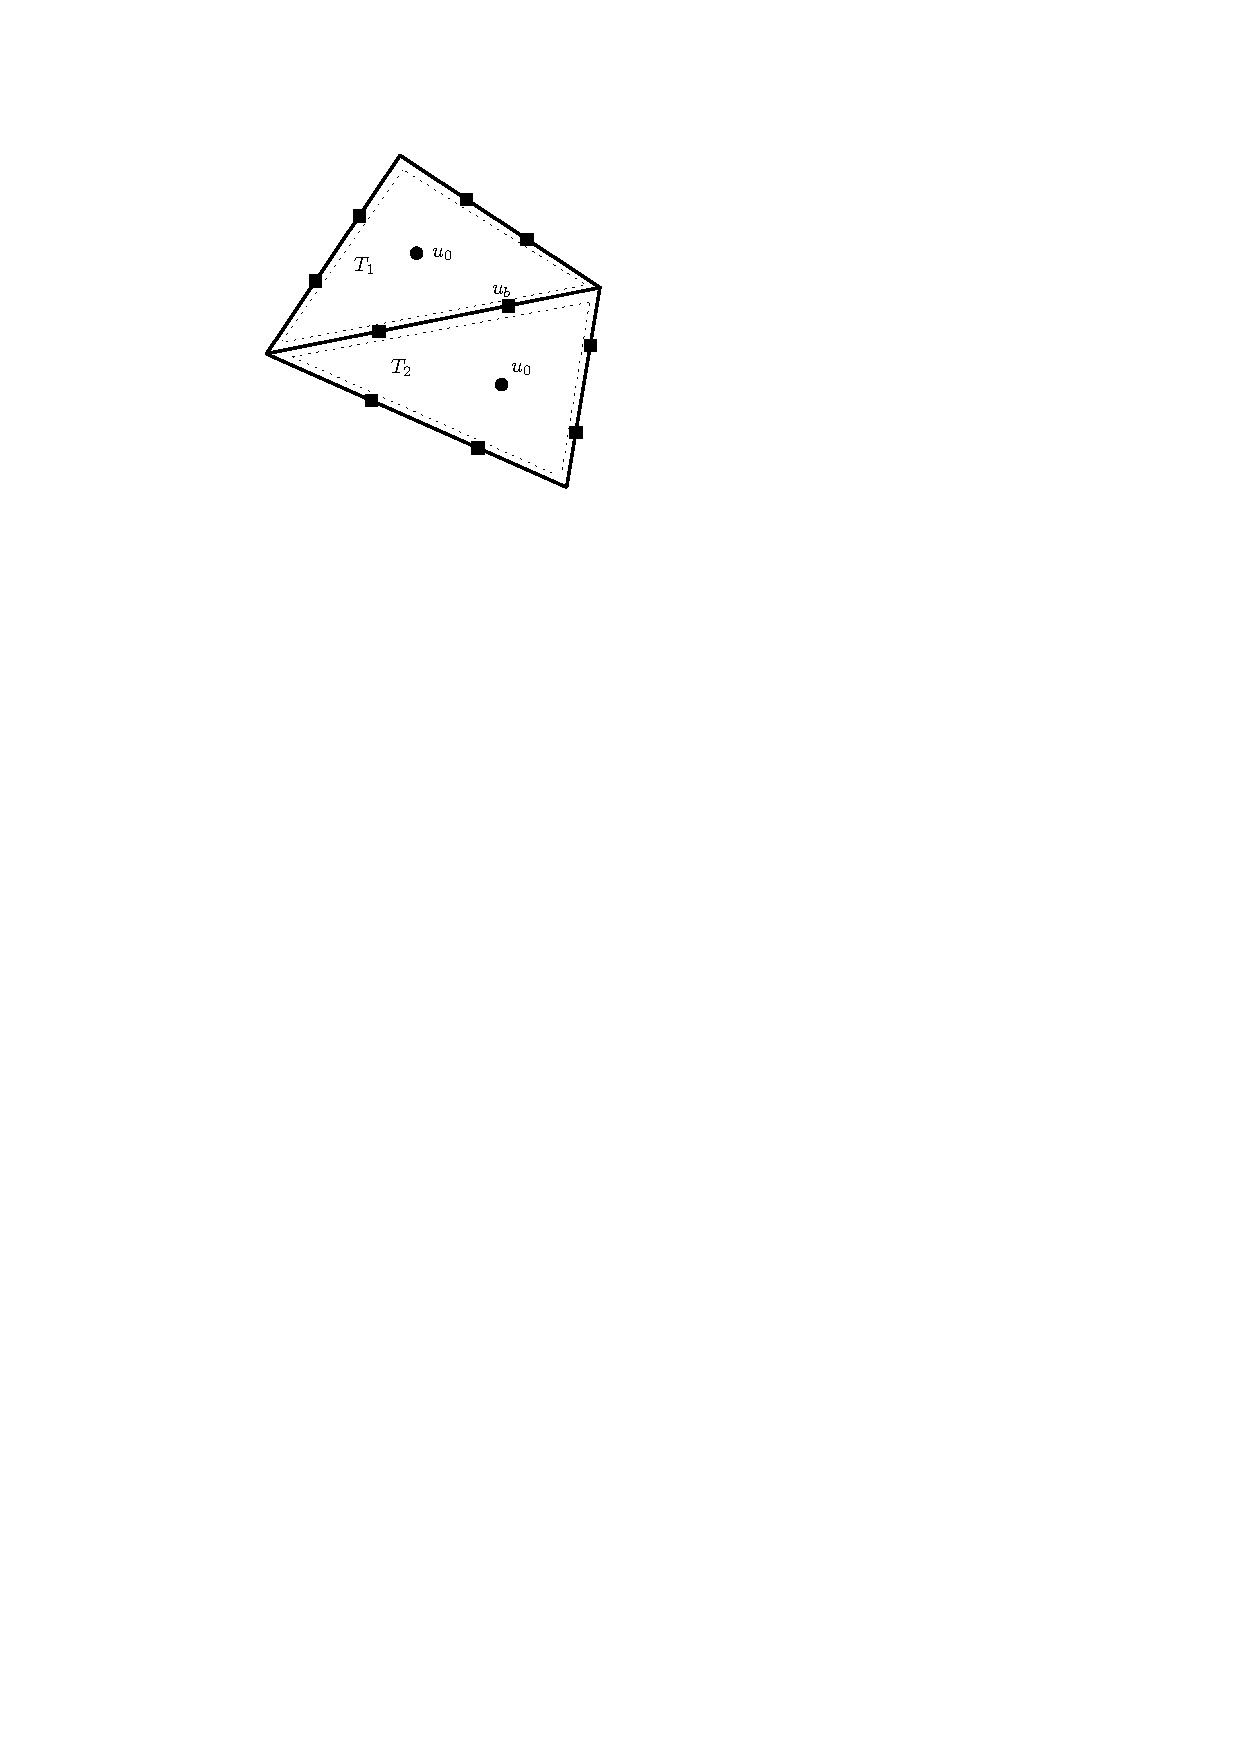
\includegraphics[width=0.4\textwidth]{./pics/triangle.pdf}
	\end{tabular}
	\caption{\footnotesize Weak Galerkin triangular elements and solution points.}\label{fig1: triangle}
\end{figure}

For Fig. \ref{fig:tri2D}, we set linear basis functions, two unknown variables, on each edge. The dash line represents the fictitious boundary of interior space. We can apply different order of polynomials on it. The two spaces are independent of each other.  

In this section, we present a triangular WG element with linear interior and boundary space. There are three interior basis functions representing the $ x, y $ and $ xy $ respectively.

\subsection{Weak Galerkin Quadrilateral Meshes}

Consider triangular element linear type basis function for both interior and boundary subspaces $ Q_{1}(T) / Q_{1} (\partial T) $
\begin{equation}
\phi_{k} = \{ \lambda_{k}, 0 \}, \qquad k = 1,2, 3
\end{equation}
\begin{equation}
\phi_{3 + l} = \{ 0, \mu_{l} \}, \qquad l = 1, 2, \cdots , 2N
\end{equation}
where N is the number of element boundaries.
\begin{figure}[H]
	\centering
	\begin{tabular}{c}
		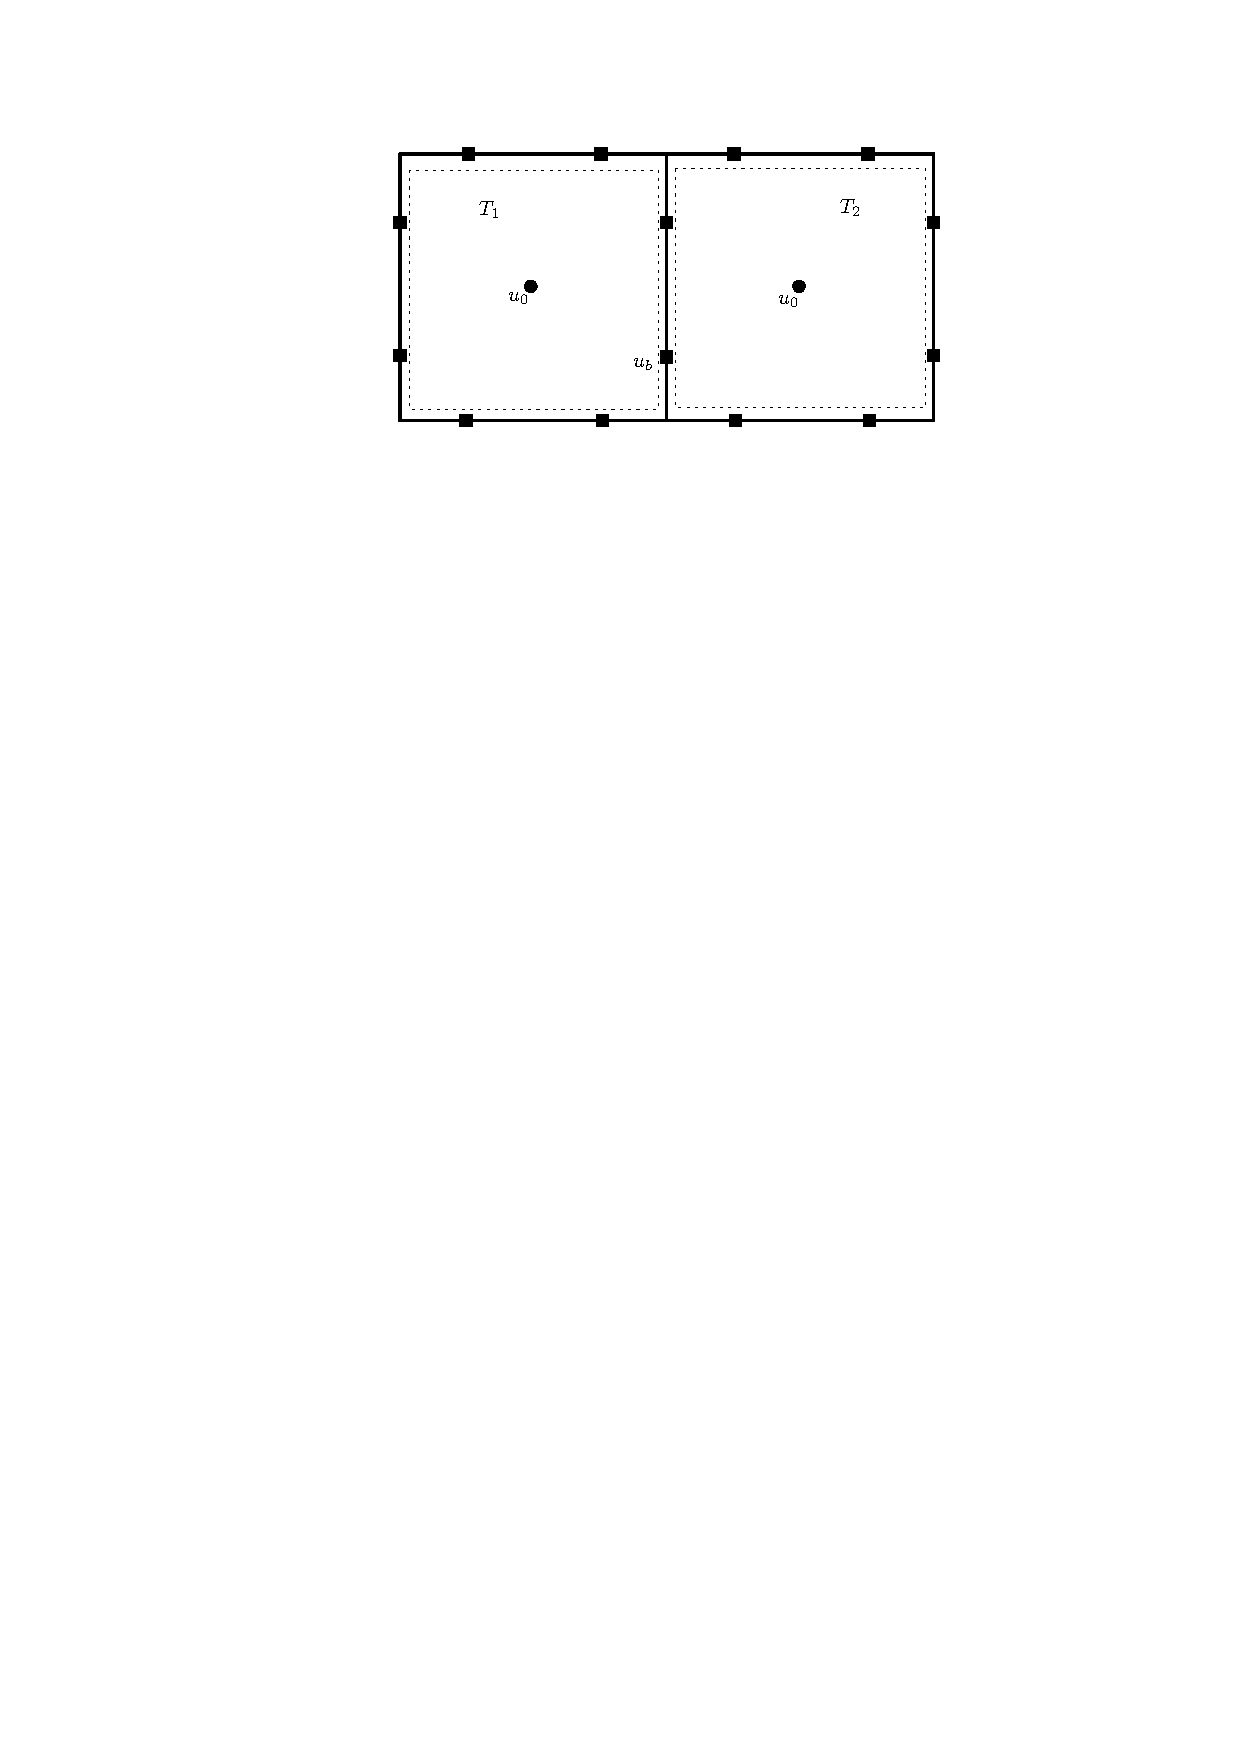
\includegraphics[width=0.8\textwidth]{./pics/quad.pdf}
	\end{tabular}
	\caption{\footnotesize Weak Galerkin quadrilateral elements and solution points.}\label{fig2: quad}
\end{figure}

In above figure, we present a quadrilateral WG element with linear interior and boundary space. There are three interior basis functions representing the $ x, y $ and $ xy $ respectively. Meanwhile, there are eight boundary basis functions represents six solution points based on the location of Gaussian points.

%---------------------------------------------------------------------------
\subsection{Numerical Examples}

We also consider the linear elasticity Equation in the square domain $ \Omega = (0, 1)^2 $. For each subdomain, it is partitioned into uniform triangular and quadrilateral mesh wish mesh size $ h $. The right-hand side function $ f $ is chosen. The exact solution is given by

\begin{equation}
u = \begin{pmatrix}
sin(2 \pi x) sin(2\pi y) \\ 1\\
\end{pmatrix}
\end{equation}

the solution is shown as below

\begin{figure}[H]
	\centering
	\begin{tabular}{c}
		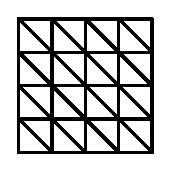
\includegraphics[width=0.4\textwidth]{./pics/triangleMesh}
	\end{tabular}
	\caption{\footnotesize Triangle mesh elements}
\end{figure}

\begin{table}[h]
	\setlength{\tabcolsep}{2pt} {
		\caption{ Numerical results for triangular element.}
		\label{Tab:hwgcg l1}
		\vspace{-5pt}
		\begin{center}
			%	\scalebox{0.6}{
			\begin{tabular}{c|c|c|c|c}
				\hline
				\multicolumn{5}{c}{\# CG = 20} \\
				\hline
				\#WG & $ E (u_{0}) $ & $ O(u_{0}) $ & $ E(u_{b})  $& $ O(u_{b})  $\\
				\hline
				$ 4 $ & $ 9.484e-2 $ & - & $ 8.484e-2 $ & - \\
				\hline
				$ 16 $ & $ 2.678e-3 $ & $ 1.9 $& $ 2.178e-3 $ & $ 1.9 $ \\
				\hline
				$ 64 $ & $ 5.570e-4 $ & $ 2.0 $ & $ 5.470e-4 $ & $ 1.9 $ \\
				\hline
				$ 256 $ & $ 1.437e-4 $ & $ 2.0 $ & $ 1.367e-4 $ & $ 2.0 $\\
				\hline
			\end{tabular}
			%	}
		\end{center} }
	\end{table}
	
	\begin{figure}[H]
		\centering
		\begin{tabular}{c}
			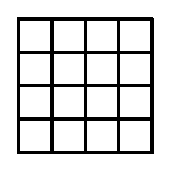
\includegraphics[width=0.4\textwidth]{./pics/quadMesh}
		\end{tabular}
		\caption{\footnotesize Quadrilateral mesh elements}
	\end{figure}
	
	
	\begin{table}[h]
		\setlength{\tabcolsep}{2pt} {
			\caption{ Numerical results for quadrilateral element.}
			\label{Tab:hwgcg l1}
			\vspace{-5pt}
			\begin{center}
				%	\scalebox{0.6}{
				\begin{tabular}{c|c|c|c|c}
					\hline
					\multicolumn{5}{c}{\# CG = 20} \\
					\hline
					\#WG & $ E (u_{0}) $ & $ O(u_{0}) $ & $ E(u_{b})  $& $ O(u_{b})  $\\
					\hline
					$ 4 $ & $ 8.368e-2 $ & - & $ 9.103e-2 $ & - \\
					\hline
					$ 16 $ & $ 1.944e-3 $ & $ 1.9 $& $ 2.058e-3 $ & $ 1.9 $ \\
					\hline
					$ 64 $ & $ 5.337e-4 $ & $ 2.0 $ & $ 5.280e-4 $ & $ 2.0 $ \\
					\hline
					$ 256 $ & $ 1.086e-4 $ & $ 2.0 $ & $ 1.451e-4 $ & $ 2.0 $\\
					\hline
				\end{tabular}
				%	}
			\end{center} }
		\end{table}
		
		\vspace{5mm}
		
		We tested the WG method for solving elasticity equation. Second order of accuracy is achieved for interior unknown variables $ u_0 $ and boundary unknown variables $ u_b $ in the triangular and quadrilateral elements.

